\documentclass{beamer}
\usetheme{Frankfurt}
% \setbeameroption{show notes}
% \setbeamertemplate{note page}[plain]

\usepackage[T1]{fontenc}
\usepackage[utf8]{inputenc}
\usepackage[french,english]{babel}

\usepackage{blindtext}
\usepackage{appendixnumberbeamer}

\usepackage{tikz}
\usetikzlibrary{positioning}
\usetikzlibrary{matrix}
\tikzset{
    invisible/.style={opacity=0,%
    prefix after command={\pgfextra{\tikzset{every label/.style={opacity=0}}}}},
    visible on/.style={alt={#1{}{invisible}}},
    alt/.code args={<#1>#2#3}{%
      \alt<#1>{\pgfkeysalso{#2}}{\pgfkeysalso{#3}}
    },
}

\title{Experiments on automation of formal verification of devices at the binary level}
\subtitle{}
\author{Thomas Lacroix}
\titlegraphic{
\includegraphics[width=4cm]{logos/insa-logo-coul.png}}
\institute{INSA Lyon \\ Soutenance de PFE (Option R\&D)}
\date{19/06/2019}

\newcommand{\htriple}[3]{\ensuremath{\{#1\}~#2~\{#3\}}}
\newcommand{\WP}{\ensuremath{\mathit{WP}}}

% Add pages before every section and subsections
\AtBeginSection[]{\frame{\sectionpage}}
\AtBeginSubsection[]
{%
    \begin{frame}
        \frametitle{Table of Contents}
        \tableofcontents[hideothersubsections, currentsection, currentsubsection]
    \end{frame}
}

% Add page number in upper-right corner
\makeatletter
\defbeamertemplate*{headline}{my smoothbars theme}
{%
    \pgfuseshading{beamer@barshade}%
    \ifbeamer@sb@subsection%
    \vskip-9.75ex%
    \else%
    \vskip-7ex%
    \fi%
    \begin{beamercolorbox}[ignorebg,ht=2.25ex,dp=3.75ex]{section in head/foot}
    \insertnavigation{.9\paperwidth}\hfill%
    \insertframenumber/\inserttotalframenumber%
    \hspace{.5em}
    \end{beamercolorbox}%
    \ifbeamer@sb@subsection%
    \begin{beamercolorbox}[ignorebg,ht=2.125ex,dp=1.125ex,%
        leftskip=.3cm,rightskip=.3cm plus1fil]{subsection in head/foot}
        \usebeamerfont{subsection in head/foot}\insertsubsectionhead
    \end{beamercolorbox}%
    \fi%
}%
\makeatother

% To remove the navigation buttons at the bottom
% \beamertemplatenavigationsymbolsempty

% Explain NIC and what we want to prove
%   - obvious reason: connected to Internet and DMA access
%   - buffer descriptor
%       - not circular
%       - only readable memory
%       - not overlapping
%   - show that it's possible to violate the invariant
%       -> overlapping tx and rx BD
%   => need to model the spec
%   => modeled with invariants
%
% Can we reuse work done for software verification to verify hardware?
%
% Start with explanation of PP analysis vs non-PP
%
% Last 5 minutes, show every supporting tools
%   => everything that is needed that is not direct PP stuff

%%%%%%%%%%%%%%%%%%%%%%%%%%%%%%%%%%%%%%%%%%%%%%%%%%%%%%%%%%%%%%%%%%%%%%%%%%%%%%%%
%%%%%%%%%%%%%%%%%%%%%%%%%%%%%%%%%%%%%%%%%%%%%%%%%%%%%%%%%%%%%%%%%%%%%%%%%%%%%%%%
%%%%%%%%%%%%%%%%%%%%%%%%%%%%%%%%%%%%%%%%%%%%%%%%%%%%%%%%%%%%%%%%%%%%%%%%%%%%%%%%

\begin{document}

\begin{frame}
    \maketitle
\end{frame}

%%%%%%%%%%%%%%%%%%%%%%%%%%%%%%%%%%%%%%%%%%%%%%%%%%%%%%%%%%%%%%%%%%%%%%%%%%%%%%%%
%%%%%%%%%%%%%%%%%%%%%%%%%%%%%%%%%%%%%%%%%%%%%%%%%%%%%%%%%%%%%%%%%%%%%%%%%%%%%%%%
%%%%%%%%%%%%%%%%%%%%%%%%%%%%%%%%%%%%%%%%%%%%%%%%%%%%%%%%%%%%%%%%%%%%%%%%%%%%%%%%

\section{Motivation}

%%%%%%%%%%%%%%%%%%%%%%%%%%%%%%%%%%%%%%%%%%%%%%%%%%%%%%%%%%%%%%%%%%%%%%%%%%%%%%%%

\subsection{Security critical systems}

\begin{frame}{Security critical systems}
    \begin{columns}
        \begin{column}{0.5\textwidth}
            Privacy

            \begin{itemize}
                \item Smartphones
                \item Smart TVs
            \end{itemize}
        \end{column}
        \begin{column}{0.5\textwidth}
            Integrity

            \begin{itemize}
                \item Hospital equipment
                \item Traffic control systems
                \item Power plants
            \end{itemize}
        \end{column}
    \end{columns}

    \vfill
    \pause

    \note{Systems are getting more and more complex with time, and}
    \textbf{Problem}: complex systems almost always contain bugs
    \note{bugs => vulnerabilities}
\end{frame}

\begin{frame}{Security critical systems - vulnerable}
    \pause
    \begin{columns}
        \begin{column}{0.5\textwidth}
            \begin{figure}
                \centering
                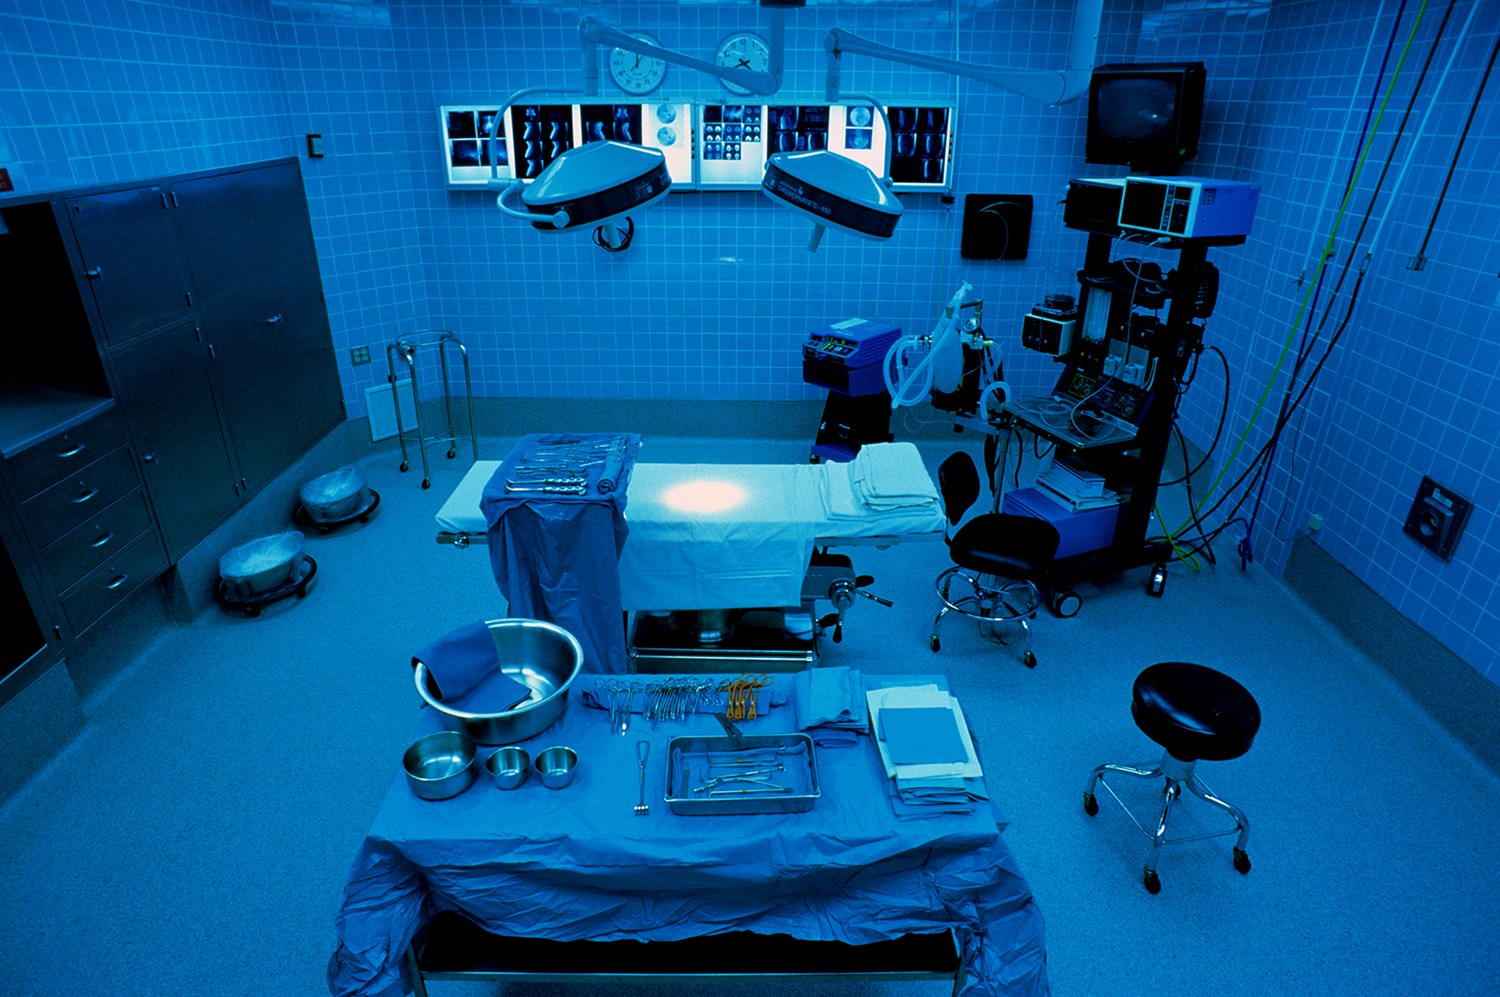
\includegraphics[height=.3\textheight]{figures/hospital-hacking.jpg}
                \caption{``It's Insanely Easy to Hack Hospital Equipment'' \cite{zetter_its_2014}}
                % zetter_its_2014: picture and article
                \label{hack_hospital}
            \end{figure}
            \pause
            \begin{itemize}
                \item Remote control of equipment
            \end{itemize}
        \end{column}
        \pause
        \begin{column}{0.5\textwidth}
            \begin{figure}
                \centering
                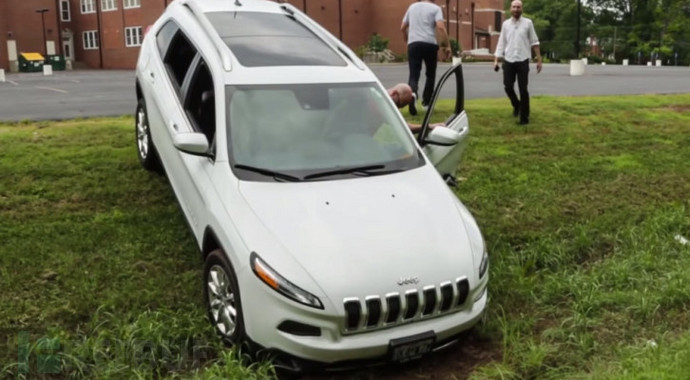
\includegraphics[height=.3\textheight]{figures/jeep_offroad.jpg}
                \caption{``Remote Exploitation of an Unaltered Passenger Vehicle'' \cite{greenberg_hackers_2015,miller_remote_2015}}
                % greenberg_hackers_2015: picture
                % miller_remote_2015: white paper
                \label{jeep_offroad}
            \end{figure}
            \pause
            \begin{itemize}
                \item Total control of drive systems
            \end{itemize}
        \end{column}
    \end{columns}
\end{frame}

% \begin{frame}{Security critical systems - vulnerable}
%     Vulnerabilities are caused by:
%     \begin{itemize}
%         \item Increased surface of attack (more and more features, codebases explode in size)
%         \item Connected to networks $\rightarrow$ remote attacks
%     \end{itemize}

%     \note{Often a result of misconfiguration.}
% \end{frame}

\begin{frame}{Secure operating systems}
    \begin{columns}
        \begin{column}{0.4\textwidth}
            \begin{center}
                
\includegraphics[height=2cm]{logos/seL4-logo-text-white.png}
            \end{center}
        \end{column}
        \pause
        \begin{column}{0.6\textwidth}
            Formal proof\footnotemark:
            \begin{itemize}
                \item The binary code correctly implements its \textbf{abstract specification}.
                \item The specification guarantees \textbf{integrity} and \textbf{confidentiality}.
            \end{itemize}

            \bigskip
            \pause

            \begin{itemize}
                \item \textbf{Integrity}: data cannot be \textit{changed} without permission.
                \item \textbf{Confidentiality}: data cannot be \textit{read} without permission.
            \end{itemize}
        \end{column}
    \end{columns}
    \footnotetext{\tiny \url{https://sel4.systems/Info/FAQ/proof.pml}}
\end{frame}

\begin{frame}{Secure operating systems}
    \begin{columns}
        \begin{column}{0.4\textwidth}
            \begin{center}
                
\includegraphics[height=2cm]{logos/seL4-logo-text-white.png}
            \end{center}
        \end{column}
        \begin{column}{0.6\textwidth}
            Proof assumptions\footnotemark:
            \pause
            \begin{itemize}
                \item Use of Direct Memory Access (DMA) is excluded, or only allowed for \textbf{trusted drivers that have to be formally verified by the user}.
            \end{itemize}

            \note{Ongoing work: IOMMUs on x86 or System MMUs on ARM.}
        \end{column}
    \end{columns}
    \footnotetext{\tiny\url{https://docs.sel4.systems/FrequentlyAskedQuestions\#is-sel4-proven-secure}}
\end{frame}

\begin{frame}
    \begin{center}
        \begin{figure}
            \only<1|handout:0>{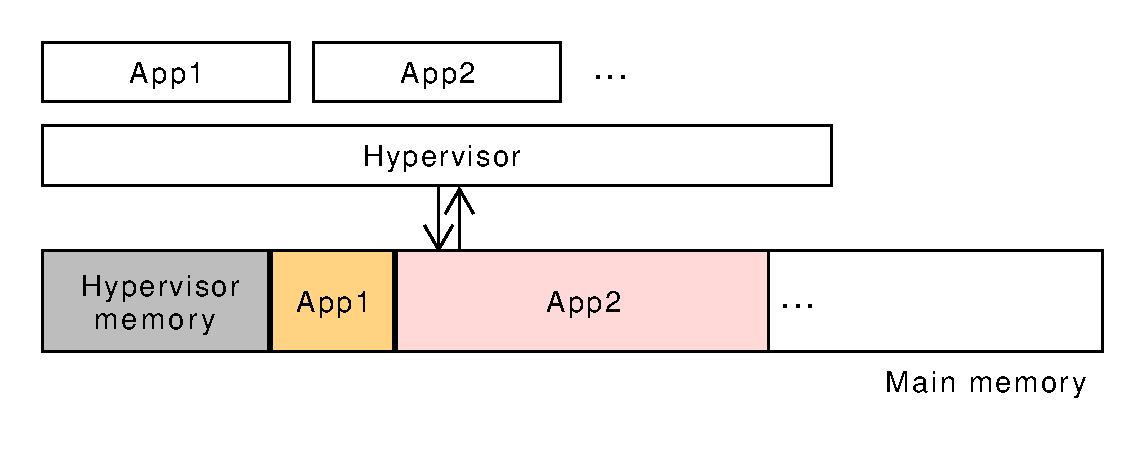
\includegraphics[width=\textwidth]{figures/dma-hyp-apps-nodma.pdf}}
            \only<2>{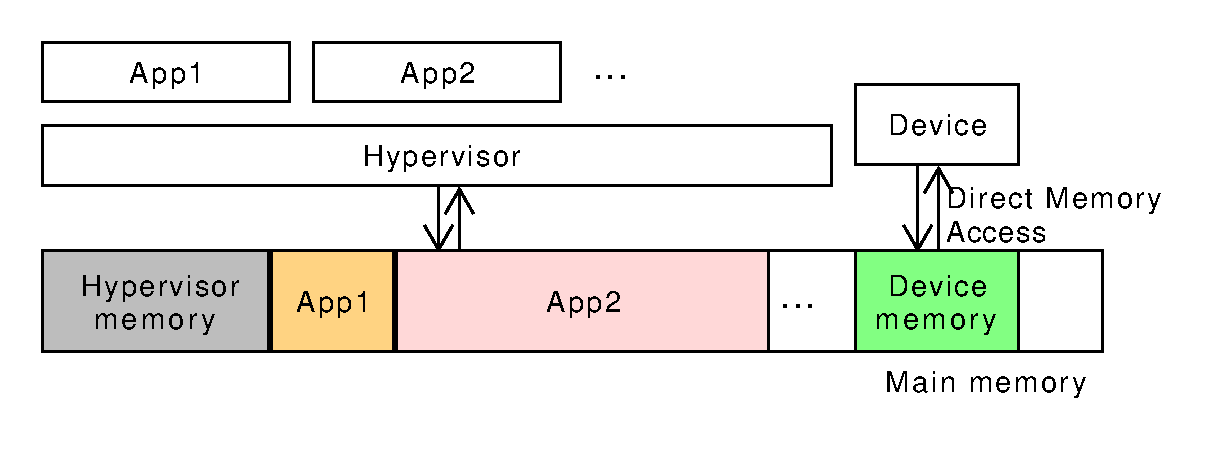
\includegraphics[width=\textwidth]{figures/dma-hyp-apps.pdf}}
            \label{dma-dangers-1}
        \end{figure}
    \end{center}
\end{frame}

%%%%%%%%%%%%%%%%%%%%%%%%%%%%%%%%%%%%%%%%%%%%%%%%%%%%%%%%%%%%%%%%%%%%%%%%%%%%%%%%

\subsection{Formal verification with HOL4}

\begin{frame}{System software verification}
    \textbf{Objective}: show absence of errors in modelisation of real systems
    \bigskip

    \begin{columns}[T]
        \begin{column}{0.5\textwidth}
            \visible<2->{
                \textbf{Formal proof \phantom{long long long title}}

                machine checkable proofs using rigorous semantic
                \phantom{needs 3 lines to align}
            }

            \bigskip
            \visible<4->{
                Use small reliable kernels \\
                $\rightarrow$ produced theorems are trustworthy
            }

            \bigskip
            \visible<6->{\textit{Examples}: HOL4, Coq, Isabelle}

            % From ITP course:
            \note{However complicated and potentially buggy your code is, if a value of type theorem is produced, it has been created through the small trusted interface. Therefore the statement really holds.}
        \end{column}
        \begin{column}{0.5\textwidth}
            \visible<3->{
                \textbf{Non proof-producing verification}

                specialized programs or procedures that check a given property
            }

            \bigskip
            \visible<5->{
                Classic bug-prone software\\
                $\rightarrow$ need tests, less trustworthy \phantom{one more line}
            }

            \bigskip
            \visible<7->{SMT solvers, model checkers}
        \end{column}
    \end{columns}

    \note{Also: model checking}
\end{frame}

%%%%%%%%%%%%%%%%%%%%%%%%%%%%%%%%%%%%%%%%%%%%%%%%%%%%%%%%%%%%%%%%%%%%%%%%%%%%%%%%

\subsection{Network Interface Controllers (NIC)}

\begin{frame}{Network Interface Controller (NIC)}
    \begin{figure}
        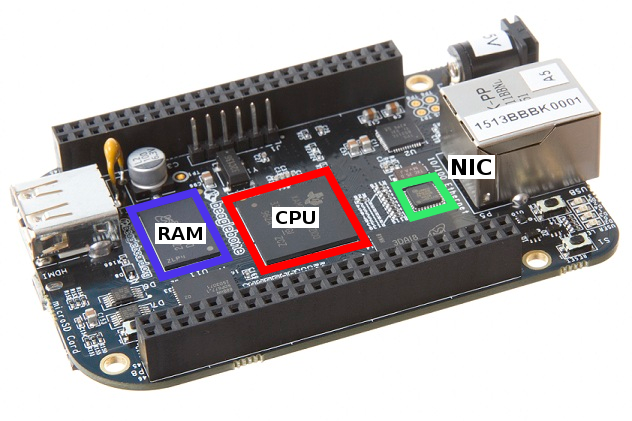
\includegraphics[]{figures/BBB_cpu_ram_nic.png}
        \caption{BeagleBone Black.}
        \label{bbb_nic}
    \end{figure}
\end{frame}

\begin{frame}{NIC: How it works}
    \begin{figure}
        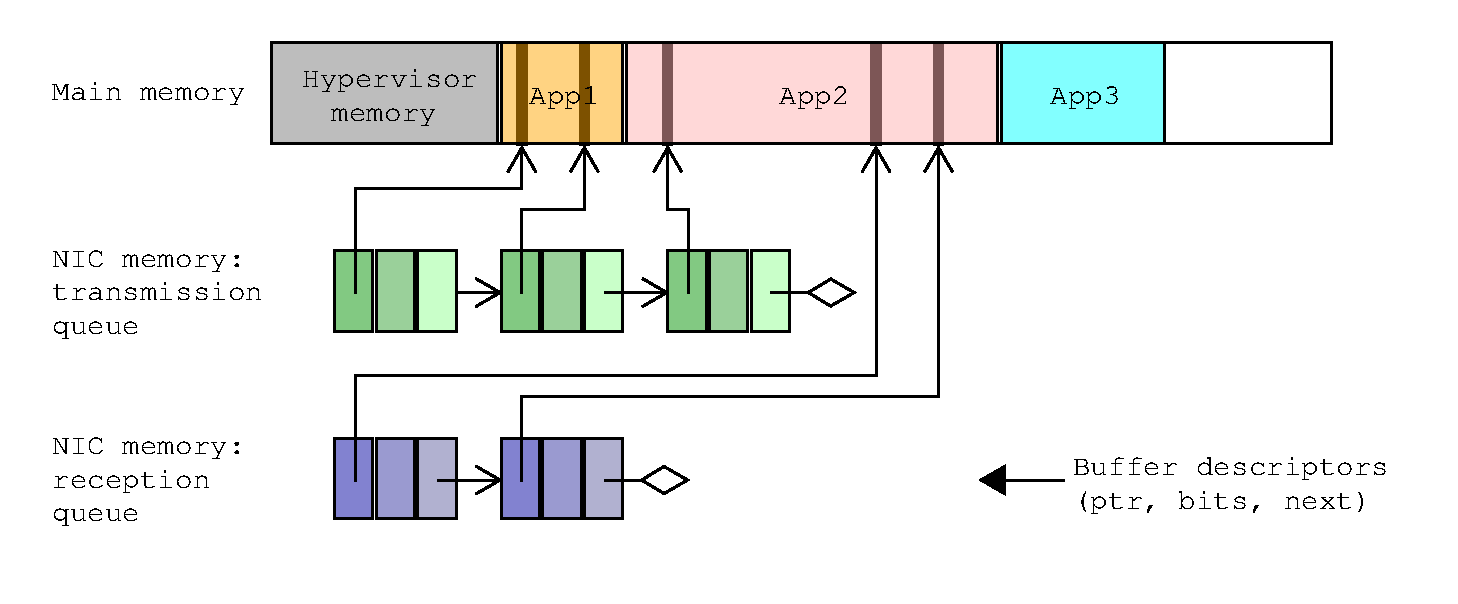
\includegraphics[width=\textwidth]{figures/nic-bd.pdf}
        \label{nic_bd}
    \end{figure}
\end{frame}

\begin{frame}{NIC: How it works}
    \begin{figure}
        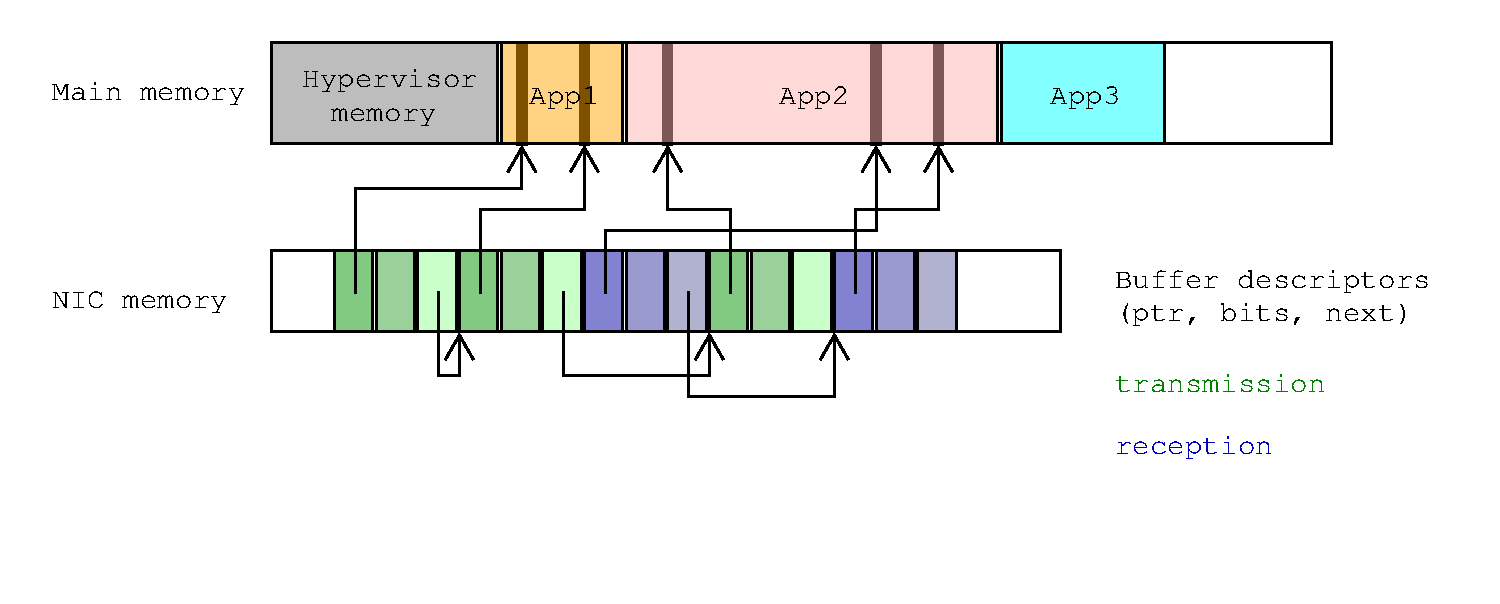
\includegraphics[width=\textwidth]{figures/nic-bd-in_mem.pdf}
        \label{nic_bd_inmem}
    \end{figure}
\end{frame}

\begin{frame}{NIC: How it can fail}
    \begin{figure}
        \includegraphics<1>[width=\textwidth]{figures/nic-bd-in_mem-overlap1.pdf}
        \includegraphics<2>[width=\textwidth]{figures/nic-bd-in_mem-overlap2.pdf}
        \includegraphics<3>[width=\textwidth]{figures/nic-bd-in_mem-overlap3.pdf}
        \label{nic_bd_inmem_overlap}
    \end{figure}
    \note{Figure 32 in Jonas' MT}
    \note{also: not circular}
\end{frame}

\begin{frame}{NIC: How it has been modeled}
    \begin{columns}
        \begin{column}{0.5\textwidth}
            \begin{center}
                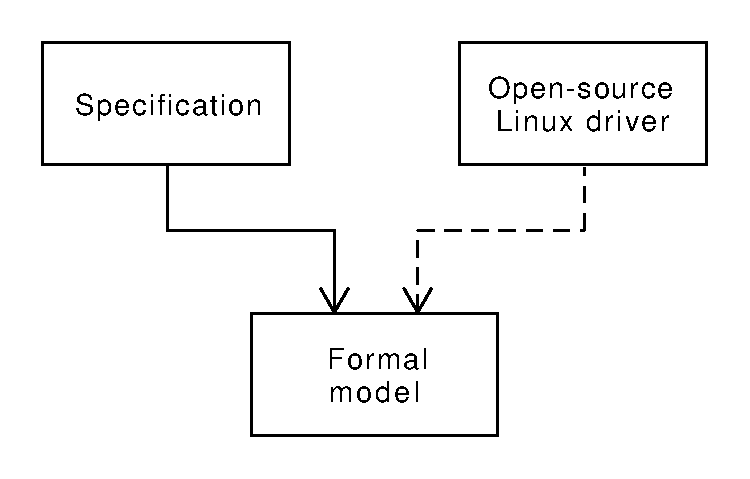
\includegraphics[width=\columnwidth]{figures/nic_how_modeled.pdf}
            \end{center}
        \end{column}
        \pause
        \begin{column}{0.5\textwidth}
            Transition system:

            \begin{center}
                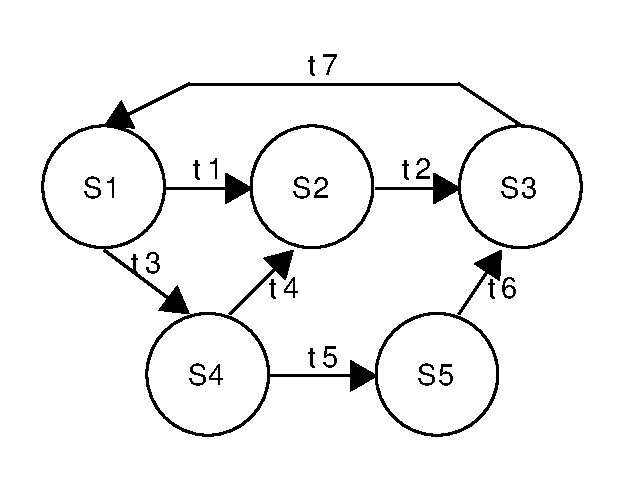
\includegraphics[width=.8\columnwidth]{figures/transition_sys.pdf}
            \end{center}

            \note{The model describes these operations to the extent that they are used by the device driver of the NIC in Linux 3.10. The NIC is modeled as a transition system where each transition corresponds to one operation that accesses one field or byte of a NIC register or the memory.}
        \end{column}
    \end{columns}
    \pause
    \begin{center}
        Unspecified behavior $\rightarrow$ ``dead'' state
    \end{center}
\end{frame}

\begin{frame}{Hoare Triple}
    \only<2>{
        \begin{center}
            \begin{tikzpicture}
                \matrix [matrix of nodes,ampersand replacement=\&, column sep=20mm]{
                    \node (a) [draw,label={P},shape=circle] {$S$}; \&
                    \node (b) [draw,label={Q},shape=circle] {$S'$}; \\
                };
                \draw[->,thick] (a) -- node[auto] {$program$} (b);
            \end{tikzpicture}
        \end{center}
    }
    \only<3->{
        \begin{center}
            \begin{equation*}
                \onslide<3->{\forall S.~P(S)}~%
                \onslide<4->{\land~S'=program(S)}~%
                \onslide<5->{\implies~Q(S')}
            \end{equation*}
        \end{center}
        \begin{columns}
            \begin{column}{.5\textwidth}
                \begin{center}
                    \begin{tikzpicture}
                        \matrix [matrix of nodes,ampersand replacement=\&, column sep=20mm]{
                            \node (a) [draw,label={P},shape=circle,visible on=<3->] {$S$}; \&
                            \node (b) [draw,label={Q},shape=circle,visible on=<5->] {$S'$}; \\
                        };
                        \draw[->,thick,visible on=<4->] (a) -- node[auto] {$program$} (b);
                    \end{tikzpicture}
                \end{center}
            \end{column}
            \begin{column}{.5\textwidth}
                \begin{center}
                    \begin{equation*}
                        \onslide<3->{\{P\}} ~ \onslide<4->{program} ~ \onslide<5->{\{Q\}}
                    \end{equation*}
                    \bigskip
                \end{center}
            \end{column}
        \end{columns}
    }
\end{frame}

\begin{frame}{Weakest precondition}
    \begin{center}
        \textit{Weakest} precondition $WP$ such that:
        \begin{equation*}
            \htriple{WP}{program}{Q}
        \end{equation*}
        \pause
        \begin{equation*}
            \Big(\forall S.~P(S) \implies WP(S)\Big) \implies \htriple{P}{program}{Q}
        \end{equation*}

        \bigskip
        \pause

        \begin{equation*}
            \WP = f(program,~Q)
        \end{equation*}
    \end{center}
\end{frame}

\begin{frame}<-8>[label=lookslike]{NIC: What the verification looks like}
    \only<8->{\setbeamercovered{transparent}}

    \uncover<2->{
        Low-level lemmas:
        \begin{itemize}
            \item<3-8> \htriple{\neg dead \land well\_configured}{transition}{\neg dead}
            \item<4-9> \htriple{\neg overlapping \land \neg cyclic}{transition}{\neg overlapping}
            \item<5-8> \htriple{\neg overlapping \land \neg cyclic}{transition}{\neg cyclic}
        \end{itemize}
    }

    \bigskip

    \uncover<6-7>{
        Intermediate lemmas:
        \begin{itemize}
            \item \textit{\small Invariant}: $rx\_invariant\_well\_defined$
            \item \textit{\small Invariant}: $tx\_invariant\_well\_defined$
        \end{itemize}
    }

    \bigskip

    \uncover<7-7>{
        Security theorems:
        \begin{itemize}
            \item $\forall~tx\_bd.~readable(tx\_bd)$ ~~~~~~~ \textit{\tiny BD = Buffer Descriptor}
            \item $\forall~rx\_bd.~writable(rx\_bd)$
        \end{itemize}
    }

    \note{Cannot express forall with BIR, and ``QF_AUFBV''}
\end{frame}
% \againframe<9>{lookslike}

\begin{frame}{Research question}
    \begin{center}
        \textbf{Can we apply traditional software verification techniques and tools to show security properties of hardware devices?}
    \end{center}
\end{frame}

\begin{frame}{HolBA: HOL4 Binary Analysis platform}
    \begin{itemize}%[<+->]
        \item Verification platform at binary level
        \item Centered around its Intermediate Language, BIR
        \item Features proof-producing tools
              \begin{itemize}
                  \item Weakest precondition generation
              \end{itemize}
    \end{itemize}
\end{frame}

%%%%%%%%%%%%%%%%%%%%%%%%%%%%%%%%%%%%%%%%%%%%%%%%%%%%%%%%%%%%%%%%%%%%%%%%%%%%%%%%
%%%%%%%%%%%%%%%%%%%%%%%%%%%%%%%%%%%%%%%%%%%%%%%%%%%%%%%%%%%%%%%%%%%%%%%%%%%%%%%%
%%%%%%%%%%%%%%%%%%%%%%%%%%%%%%%%%%%%%%%%%%%%%%%%%%%%%%%%%%%%%%%%%%%%%%%%%%%%%%%%

% \section{Automatic contract-based verification pipeline}
\section{Contract-based verification}

\subsection{Pipeline}

% \begin{frame}<1>[label=pipeline]{Contract-base verification pipeline}
%     \begin{center}
%         \includegraphics<1>[height=.8\textheight]{figures/pipeline-1.pdf}
%         \includegraphics<2>[height=.8\textheight]{figures/pipeline-2.pdf}
%         \includegraphics<3>[height=.8\textheight]{figures/pipeline-3.pdf}
%     \end{center}
% \end{frame}

\begin{frame}{Contract-based verification pipeline}
    \begin{columns}
        \begin{column}[T]{.5\textwidth}
            % \onslide<2->{
            %     \begin{center}
            %         $\{\neg dead \land well\_configured\}$\\
            %         $~tx6~$\\
            %         $\{\neg dead\}$
            %     \end{center}
            % }
            % $\WP(tx6,~\neg dead)$

            \begin{enumerate}
                \item[0.]<1-> Translate the model in BIR
                \item[1.]<2-> Formulate a Hoare Triple
                \item[2.]<3-> Translate P and Q to BIR
                \item[3.]<4-> Generate the WP
                \item[4.]<7-> Translate the goal into a SMT-compatible expression
            \end{enumerate}

            \bigskip
            \begin{center}
                \only<1>{$transition_{BIR}$}
                \only<2>{\htriple{P}{transition_{BIR}}{Q}}
                \only<3>{\htriple{P_{BIR}}{transition_{BIR}}{Q_{BIR}}}
                \only<4>{$P_{BIR}(S) \implies \WP_{BIR}(S)$}
                \only<5>{
                    \textbf{S}atisfiability \textbf{M}odulo \textbf{T}heories
                    \begin{itemize}
                        \item external tools \phantom{left left}
                        \item SMT-LIB 2.0
                    \end{itemize}
                }
                \only<6>{
                    $\neg\Big(P_{BIR}(S) \implies \WP_{BIR}(S)\Big)$
                    \bigskip

                    ``unsat''?
                }
                \only<7>{
                    $\neg\Big(P(S) \implies \WP(S)\Big)_{SMT}$
                    \bigskip

                    ``unsat''?
                }
            \end{center}
        \end{column}
        \begin{column}[T]{.6\textwidth}
            \vspace{-1cm}
            \begin{center}
                \includegraphics<1>[height=.8\textheight]{figures/pipeline-0.pdf}
                \includegraphics<2>[height=.8\textheight]{figures/pipeline-1.pdf}
                \includegraphics<3>[height=.8\textheight]{figures/pipeline-2.pdf}
                \includegraphics<4>[height=.8\textheight]{figures/pipeline-3.pdf}
                \includegraphics<5>[height=.8\textheight]{figures/pipeline-3-1.pdf}
                \includegraphics<6>[height=.8\textheight]{figures/pipeline-4.pdf}
                \includegraphics<7>[height=.8\textheight]{figures/pipeline-all.pdf}
            \end{center}
        \end{column}
    \end{columns}
\end{frame}

\subsection{How trustful is it?}

\begin{frame}{How trustful is it?}
    \begin{columns}
        \begin{column}{.5\textwidth}
            \begin{itemize}
                \setlength\itemsep{1em}
                \item<2-> SMT solver don't produce proofs
                \item<3-> bir2bool isn't proof-producing
                \item<4-> The BIR model may be wrong
            \end{itemize}
        \end{column}
        \begin{column}{.6\textwidth}
            \begin{center}
                \includegraphics<1>[height=.8\textheight]{figures/pipeline-all.pdf}
                \includegraphics<2>[height=.8\textheight]{figures/pipeline-all-trustful-1.pdf}
                \includegraphics<3>[height=.8\textheight]{figures/pipeline-all-trustful-2.pdf}
                \includegraphics<4>[height=.8\textheight]{figures/pipeline-all-trustful-3.pdf}
            \end{center}
        \end{column}
    \end{columns}
\end{frame}

\subsection{How powerful is it?}

\begin{frame}{How powerful is it?}
    \begin{block}{Not proof-producing}
        Easier non-proof producing platforms exist
    \end{block}
    \pause
    \begin{block}{Limited by SMT solvers' logics}
        \begin{itemize}
            \item<3-> \htriple{\neg overlapping \land \neg cyclic}{transition}{\neg overlapping}
            \item<4-> Logic: \textbf{QF}\_AUFBV $\rightarrow$ \textbf{Q}uantifier-\textbf{F}ree
        \end{itemize}
    \end{block}
    \pause
    \begin{block}{Cannot compose theorems}
        \begin{itemize}
            \item<6-> HolBA limitation
            \item<7-> Need theorems to compose trustfully
        \end{itemize}
    \end{block}
\end{frame}

\section{Proof-producing verification}

\subsection{Subsection 1}

\begin{frame}{Title}
\end{frame}

%%%%%%%%%%%%%%%%%%%%%%%%%%%%%%%%%%%%%%%%%%%%%%%%%%%%%%%%%%%%%%%%%%%%%%%%%%%%%%%%
%%%%%%%%%%%%%%%%%%%%%%%%%%%%%%%%%%%%%%%%%%%%%%%%%%%%%%%%%%%%%%%%%%%%%%%%%%%%%%%%
%%%%%%%%%%%%%%%%%%%%%%%%%%%%%%%%%%%%%%%%%%%%%%%%%%%%%%%%%%%%%%%%%%%%%%%%%%%%%%%%

\section{Conclusion}

\begin{frame}
    \begin{center}
        \huge
        Questions
    \end{center}
\end{frame}

%%%%%%%%%%%%%%%%%%%%%%%%%%%%%%%%%%%%%%%%%%%%%%%%%%%%%%%%%%%%%%%%%%%%%%%%%%%%%%%%
%%%%%%%%%%%%%%%%%%%%%%%%%%%%%%%%%%%%%%%%%%%%%%%%%%%%%%%%%%%%%%%%%%%%%%%%%%%%%%%%
%%%%%%%%%%%%%%%%%%%%%%%%%%%%%%%%%%%%%%%%%%%%%%%%%%%%%%%%%%%%%%%%%%%%%%%%%%%%%%%%

\appendix

\begin{frame}[allowframebreaks]{References}
    \nocite{*}
    \bibliography{ref-slides}
    \bibliographystyle{plain}
\end{frame}

\begin{frame}{Other tools for software verification}
    \textbf{TODO}: Jonas' MT, page 46 Section 2.5.4
\end{frame}
\end{document}